
\subsection{Scalability in terms of number of independent tasks}
\label{nr_machines}



\begin{figure*}[!t]
\begin{center}
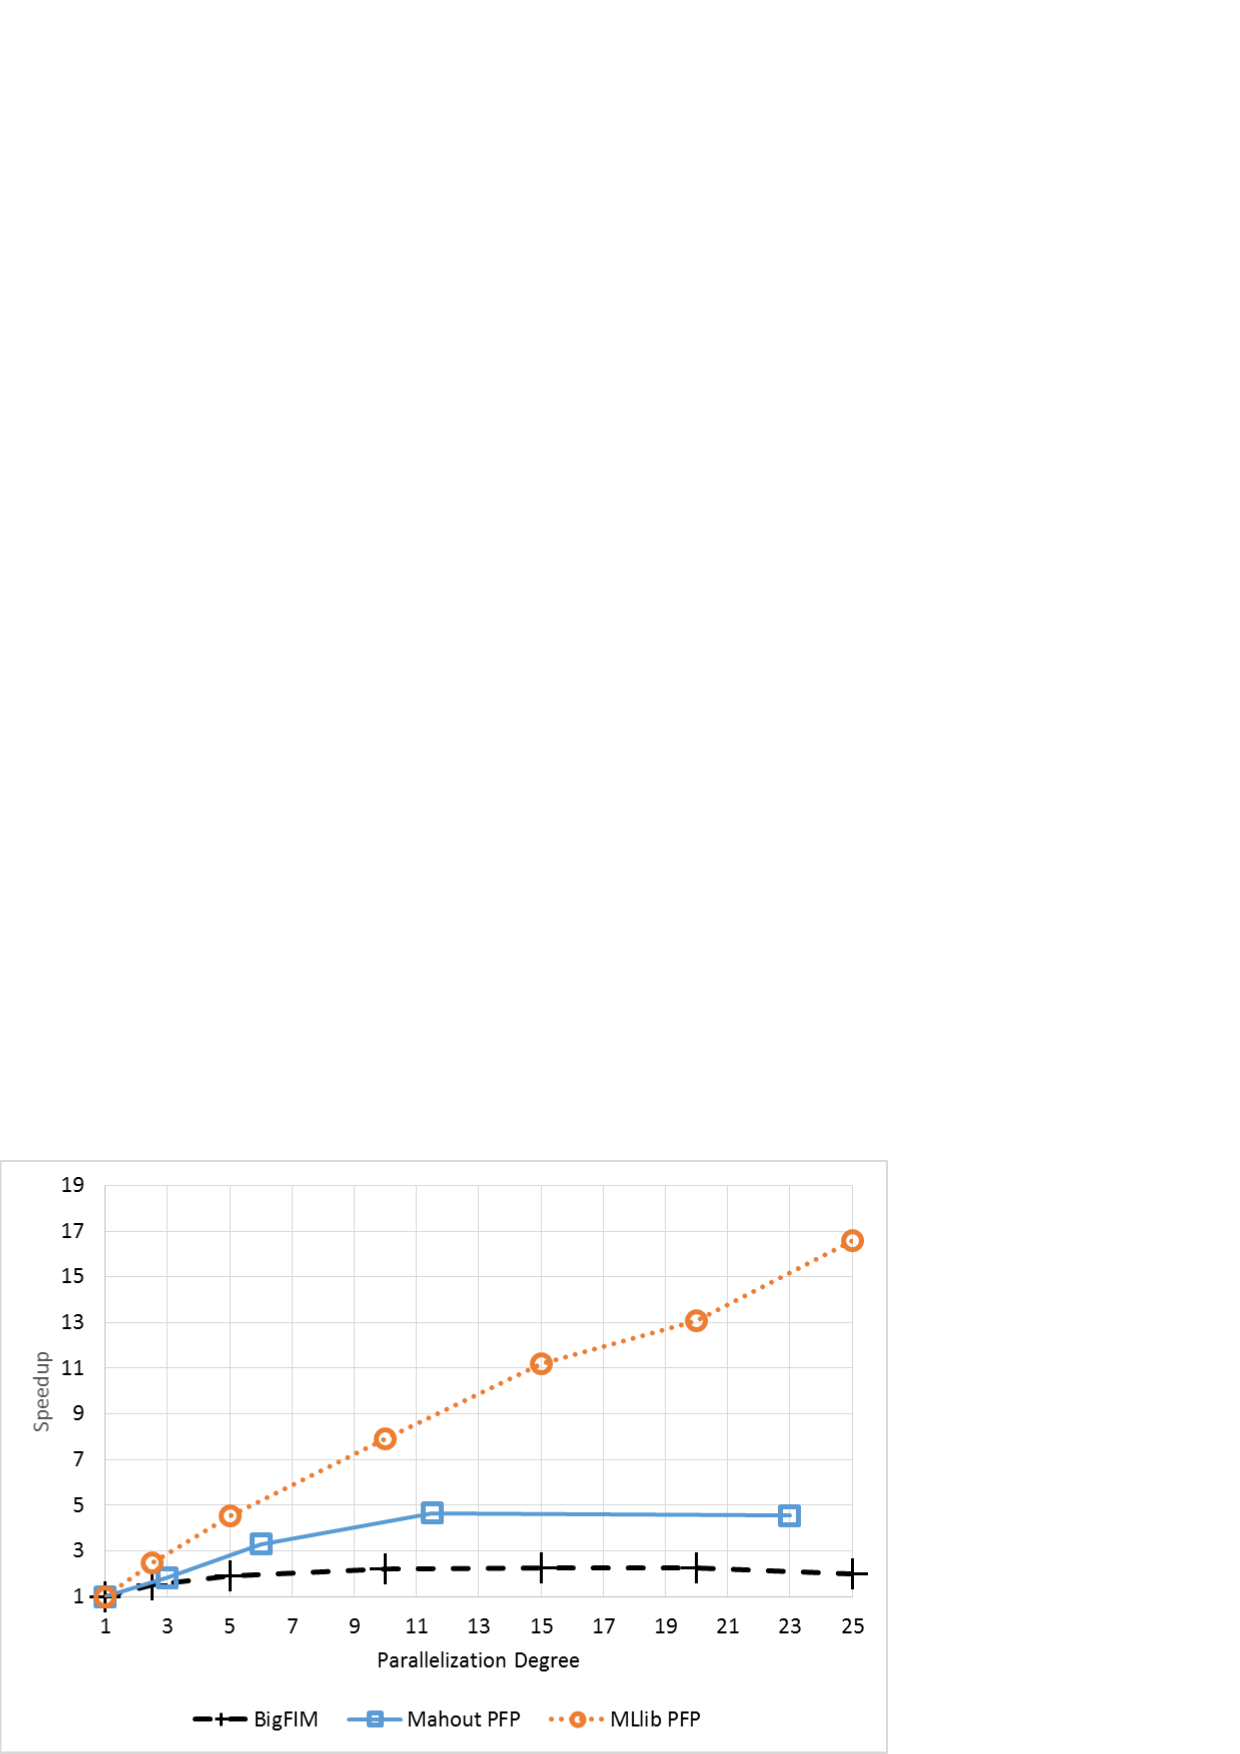
\includegraphics[width=5in]{immagini/machines_speedup.png}
\caption{Speedup with different parallelization degrees (Dataset \#12,
 $minsup$~0.15\%,
 average transaction length~10)}
\label{nr_machines_speedup}
\end{center}
\end{figure*}


%\begin{figure*}[!t]
%\begin{center}
%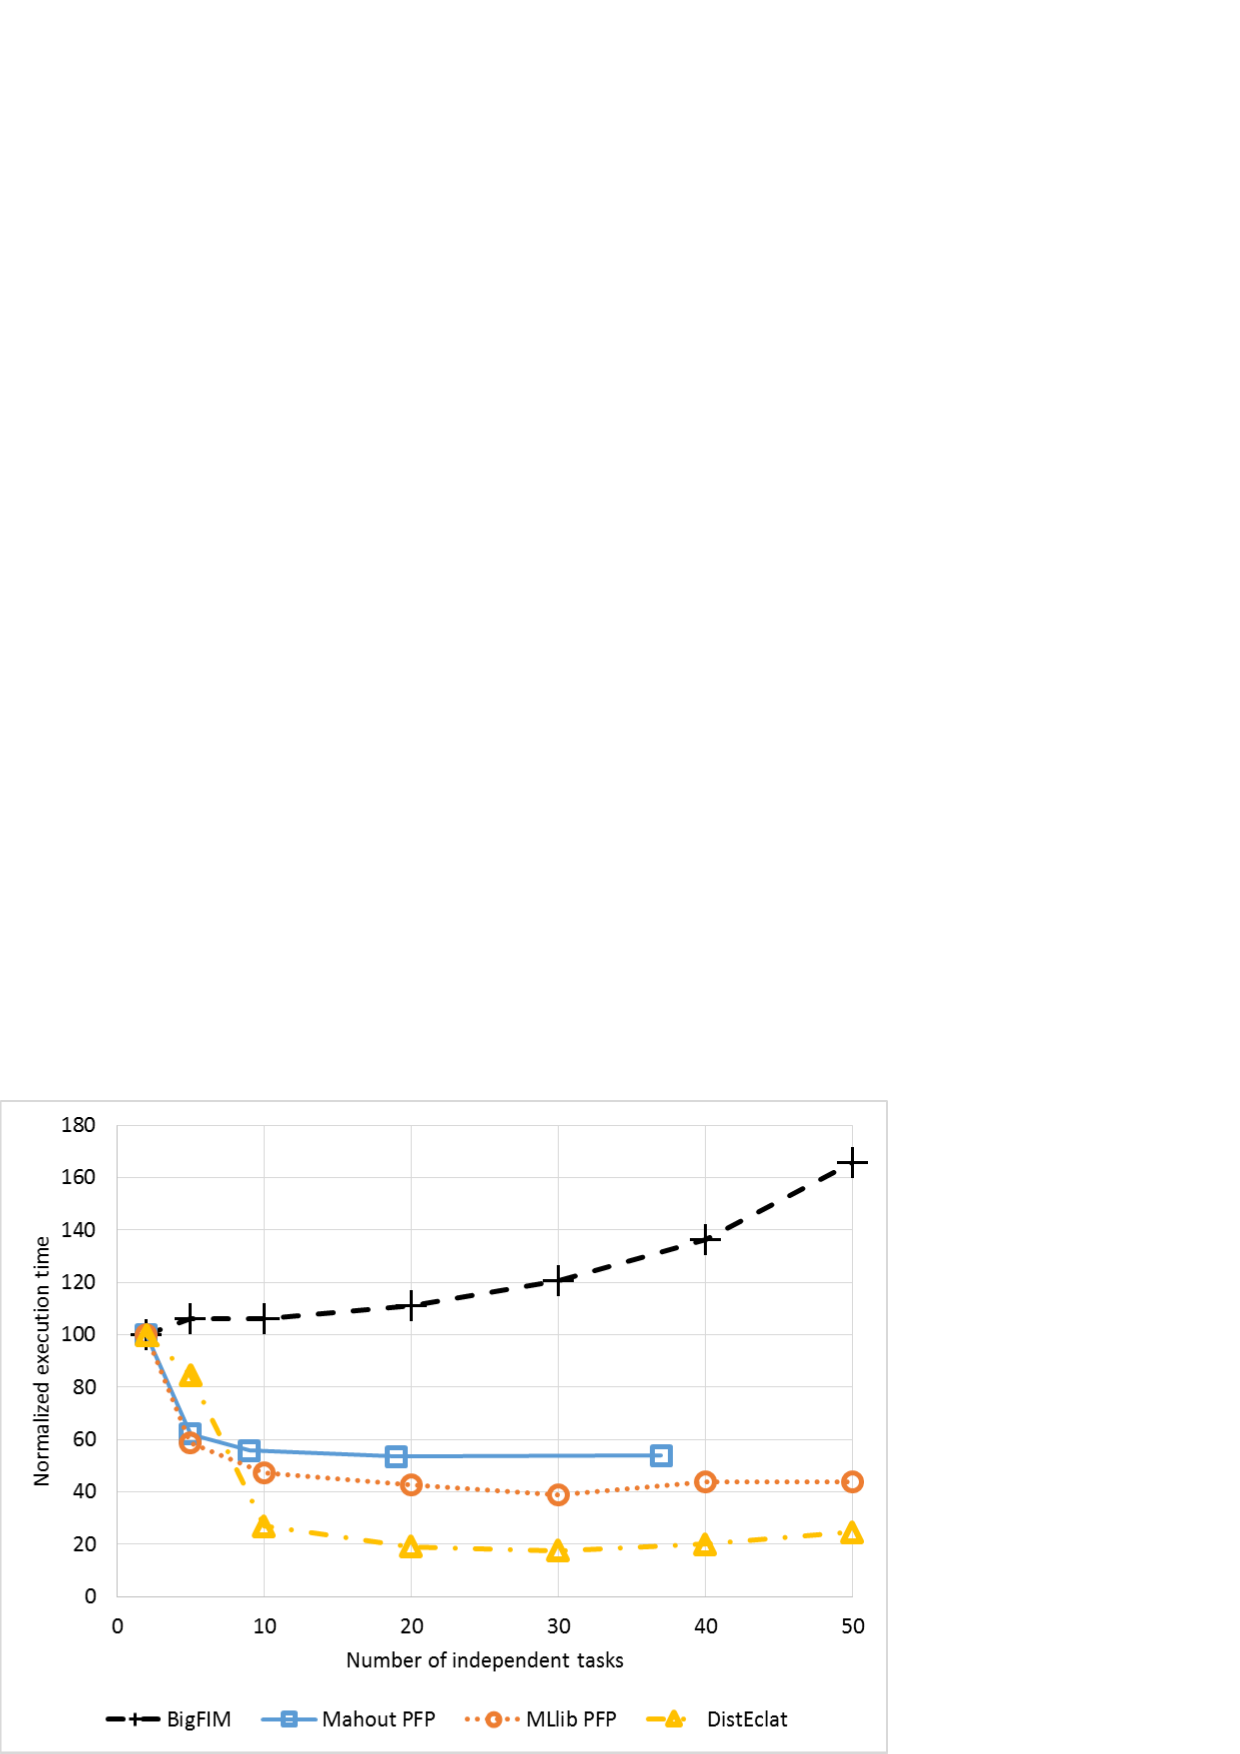
\includegraphics[width=5in]{immagini/machines_2.png}
%\caption{Normalized execution time with different number of machines  (Dataset \#1,
% $minsup$~0.11\%,
% average transaction length~10) \textbf{Qui BigFIM va proprio male, mi chiedo se sia il caso di eliminare questo esperimento (ma perderemmo disteclat)}}
%\label{nr_machines_2}
%\end{center}
%\end{figure*}

In this experiment we have evaluated the impact of the parallelization degree to the algorithms performances. Specifically, we run the same mining task with increasing degree of parallelization in terms of computational resources availability (i.e. number of parallel independent tasks). For this experiment, the parameter tuning is not trivial since it is not easy to find a mining allowing, at the same time, all the algorithms to complete it with just few machines, and deep enough not to be easily dominated by distribution overheads. We focus on a problem characterized by a large input file (Dataset \#12) and a relatively low minsup value (0.15\%) (Figure~\ref{nr_machines_1}). 
%Since the problem was already too challenging for a single task, we have started from 2. In Figure~\ref{nr_machines_1} and Figure~\ref{nr_machines_speedup} are shown the performance of the algorithms leveraging different parallelization degree values.
% In In Figure~\ref{nr_machines_1}, the execution times are normalized with respect with the execution time obtained with the time obtained with the base number of machines (i.e. 2).
In Figure~\ref{nr_machines_speedup}, the execution time of the basic configuration are divided by the ones related to the higher degree of parallelization to obtain the speedup values
% ( $T_{old}/T_{new}$ ).
%for different multiplicative factors of computation improvement (since the basic parallelization degree is 2, the number of independent tasks in the x axis can be obtained by multiplying times 2)     \footnote{Please note that the Mahout-PFP curve in Figure~\ref{nr_machines_1} appears shifted with respect to the others because of the following reason. This specifical implementation does not allow to control the numbers of mappers involved in the computation, therefore we had to change input chunk size. This value allowed us to force a fixed set of possible configurations. }. 

In this experiment, it is clear that the FP-Growth based implementations show a better scalability. BigFIM, on the contrary, is not able to leverage a high number of computing nodes. 
Because of the size of the dataset, DistEclat is not able to perform the mining. In the previous experiments, it has demonstrated to be reliable only with mining requiring less than few minutes \footnote{Considering just the experiments in which all the algorithms complete the mining}. Repeating the same kind of scalability experiment for a mining of few minutes is not sensed because the parallelization overheads likely dominate the computation.\\
%
%Since DistEclat is not able to run this experiment, we used a smaller input file (Dataset \#1) and an even lower minsup value (0.11\%) (Figure~\ref{nr_machines_2}). Even in this case, the Breadth-first approaches (DistEclat) showed a very good scalability. BigFIM demonstrated again to have serious problems of scalability. In this experiment, in fact, the problem configuration is such that the best execution times is provided with the smaller number of computing nodes. Actually, the mining phase is quite fast (about 6 minutes), with a concrete possibility, hence, to be dominated by distribution overheads, especially with Apriori iterative nature. However, a slightly deeper minsup value leads to memory issue.\\
\textbf{Discussion:}
In this Section, as predictable, it is clear that the benefits of the parallelization strongly mitigate after few tens of tasks. MLlib PFP has demonstrated to be the best approach, probably because a finest granularity in the projection of the FP-trees than the other approaches tree structures (the more are the independent structures to be mined, the better could be distributed to a high number of nodes). 
The motivations behind this difficulties are related to the Frequent itemset mining problem, which is hardly parallelizzable. The partitions to which the problem is divided into often overlap. This leads to an overall load which is higher than load of an hypothetical centralized execution. For this reason, when the exploration of the search space deepen, the overlapping of the subproblems increases and the performances do not scale as desirable. 
%\textbf{(ANCHE QUI FORSE POTREMMO ENFATIZZARE IL FATTO CHE PURTROPPO IN QUESTO DOMINIO SI SCALA DAVVERO POCO. NON CONTINUARE A GUADAGNARE ALL'INFINITO E' LA NORMA, MA QUI ANCHE PROBLEMI MOLTO GRANDI SI FERMANO DOPO QUALCHE DECINE DI MACCHINE. CI POTREMMO ALLACCIARE ALLE RIFLESSIONI FINALI IN CUI DICIAMO CHE SI VEDE CHE QUESTI SONO PORTING E NESSUNO E' STATO DAVVERO PROGETTATO PER ANDARE DIRETTAMENTE PARALLELO.}